\documentclass{article}
% \documentclass[twocolumn]{article}

\title{Batch Mapping in Mixnets}

\author{Aiswarya Walter, Student ID: 427199}

\date{}

%%packages
\usepackage[margin=1.5cm,nohead]{geometry}
\usepackage{graphicx}
\usepackage{dblfloatfix} 
\usepackage{amsmath}
\usepackage[colorlinks=true, allcolors=blue]{hyperref}
\usepackage{algorithm}
\usepackage{algpseudocode}
\usepackage{float} 
\algnewcommand\algorithmicforeach{\textbf{for each}}
\algdef{S}[FOR]{ForEach}[1]{\algorithmicforeach\ #1\ \algorithmicdo}
\usepackage{caption}  
\usepackage{afterpage}
\usepackage{placeins}  % For \FloatBarrier
\usepackage{needspace}

% Float parameters
\renewcommand{\topfraction}{0.9}
\renewcommand{\bottomfraction}{0.8}
\setcounter{topnumber}{2}
\setcounter{bottomnumber}{2}
\setcounter{totalnumber}{4}
\renewcommand{\dbltopfraction}{0.9}
\setcounter{dbltopnumber}{2}

\begin{document}

\maketitle

\section{Problem Definition}
\label{sec:problem}

Mix networks (mixnets) are anonymous communication systems that 
provide privacy protection by preventing 
adversaries from tracing communication patterns and 
linking senders to recipients. Unlike low-latency 
systems such as Tor, mixnets introduce deliberate 
delays and message mixing strategies to ensure 
 unlinkability even against powerful 
adversaries capable of global network monitoring. 
They operate by routing messages through a series 
of intermediary nodes known as mixes, which 
shuffle and delay packets to disrupt any 
correlation between input and output messages, 
making it difficult for observers to correlate 
incoming and outgoing traffic patterns.

One critical challenge in mixnet design is handling node failures, which 
can compromise message delivery and system reliability. One of the strategies 
to address this challenge is message splitting, where a single  
message is divided into multiple sub-messages that are sent as a batch. 
The original message can only be reconstructed when all sub-messages in 
the batch are successfully received at the destination. This approach 
provides fault tolerance while maintaining the mixing properties of 
the network.

The challenge arises when a global adversary observes 
the mixnet system. Such an adversary can monitor all incoming and outgoing 
traffic at the mix nodes, recording message arrival and departure timestamps, 
batch compositions, and routing patterns. This batch-level 
correlation problem is particularly challenging because 
temporal patterns, batch sizes, and network timing constraints can leak 
information about the mapping between input and output batches. Even 
though individual messages within batches may be cryptographically 
protected, the observable metadata (timing, message counts) 
can be exploited to reduce the anonymity provided by the mixnet.

\textbf{Problem Statement:} Given a mixnet system operating with fixed-size 
message batches under observation by a global adversary, the aim is to develop 
an algorithm that computes the probability 
that each observed outgoing batch corresponds to each possible incoming 
batch, considering timing constraints and batch coherence requirements.

\section{Proposed Solution: The Mixnet Batch Matching Algorithm}
\label{sec:solution}

The Mixnet Batch Matching algorithm addresses the batch 
correlation problem by systematically enumerating 
all valid message-to-batch mappings and computing 
probability distributions for each outgoing batch. 
The algorithm operates incrementally, processing 
each outgoing message as it enters a batch and 
updating the global set of valid permutations 
while maintaining temporal and batch coherence 
constraints.

Table~\ref{tab:variables} provides a comprehensive 
overview of the key variables, data structures, 
and functions used throughout the algorithm. 
The algorithm maintains several core data 
structures: \texttt{Valids} stores the current 
set of valid permutations, \texttt{OutBatchMappingCount} 
tracks the number of valid mappings for each 
outgoing-incoming batch pair, \texttt{BatchProb} 
contains the final probability distributions, 
and \texttt{OutMsgMappingSet} holds the eligible 
incoming messages for each outgoing batch. The algorithm 
also maintains anonymity-related structures: 
\texttt{AnonymitySet} stores the set of incoming batches 
that could have contributed to each outgoing batch, 
while \texttt{AnonymitySetSize} records the cardinality 
of these anonymity sets for privacy quantification. 
The helper functions \texttt{batchid()} and \texttt{msgid()} 
extract batch and message identifiers respectively, 
while \texttt{appendMsg()} handles the creation of 
extended sub-permutations during the permutation 
expansion phase.

The following subsections describe each phase of the algorithm in detail, providing both pseudocode and comprehensive explanations of the underlying logic.

% \vspace{1em} 
\begin{table*}[!htbp]
\centering\footnotesize 
\begin{tabular}{l p{5.5cm} p{5.5cm}}
\hline
\textbf{Variables and Functions} & \textbf{Description} & \textbf{Data Type} \\
\hline
$M_{ij}$      & $j$-th message in the incoming batch $i$ & Message object\\
$O_{pq}$      & $q$-th message in the outgoing batch $p$ & Message object\\
$t_{M_{ij}}$  & Arrival time of message $M_{ij}$ & Timestamp  \\
$t_{O_{pq}}$  & Sending time of message $O_{pq}$ & Timestamp  \\
$IncomingBatches$ & Mapping of incoming batch ids to its messages & Dictionary of dictionaries \\
$OutgoingBatches$ & Mapping of outgoing batch ids to its messages & Dictionary of dictionaries \\
$OutBatchMappingCount$ & For each outgoing batch, it maps the candidate incoming batches to the number of valid permutations to that batch & Dictionary of dictionaries \\
$OutMsgMappingSet$ & Set of valid input messages for each outgoing batch, $C_{p}$ & Dictionary of sets of messages \\
$Valids$      & List of valid message permutations for all outgoing batches & List of dictionaries of lists  \\
$BatchProb$ & Probability mapping for all output batches & Dictionary of dictionaries \\
$AnonymitySet$ & Set of messages that contribute to the anonymity of each outgoing batch & Dictionary of sets of messages \\
$AnonymitySetSize$ & Number of incoming batches that could have contributed to each outgoing batch & Dictionary of integers \\
$batchid(msg)$ & Returns the batch id of the message  & Function (returns integer) \\
$msgid(msg)$   & Returns the message id  & Function (returns integer) \\
$appendMsg(subpermutation, msg)$  & Operation to append a message to an existing sup-permutation of a batch  & Function (returns list) \\
\hline
\end{tabular}
\caption{Algorithm variables and functions.} % (add a caption; helps placement)
\label{tab:variables}
\end{table*}
\vspace{1em} 

\subsection{Initialization and Candidate Selection}

This initialization phase sets up the fundamental 
data structures and identifies eligible messages 
for batch mapping. The algorithm first initializes 
empty containers for valid permutations, 
batch probabilities, and anonymity metrics, 
then determines which incoming batches are 
candidates for mapping to the current outgoing 
batch based on size constraints ($lenIn \geq lenOut$), 
and finally collects all incoming messages that 
satisfy the temporal constraint ($t_{M_{ij}} < t_{O_{pq}}$) 
for subsequent processing.

\begin{algorithm}[H]
\caption*{Phase 1: Initialization and Candidate Selection}
\begin{algorithmic}[1]
\State $Valids \gets [] $
\State $BatchProb \gets \{ \} $
\State $ AnonymitySet \gets \{ \} $
\State $ AnonymitySetSize \gets \{ \} $
\State Outgoing message $O_{pq}$ enters the outgoing batch, $p$ at time $t_{O_{pq}}$
\State $OutMsgMappingSet [p] \gets \{ \} $
\ForEach{$ i \text{ in } IncomingBatches $}
    \State $ lenIn \gets len(IncomingBatches[i]) $
    \State $ lenOut \gets len(OutgoingBatches[p]) $
    \If{$ lenIn \geq  lenOut $}
        \State $OutBatchMappingCount[p][i] \gets 0 $
    \EndIf
\EndFor
\ForEach{$ i \text{ in } OutBatchMappingCount[p] $}
    \ForEach{$ M_{ij}, t_{M_{ij}} \text{ in } IncomingBatches[i] $}
        \If{$ t_{M_{ij}} < t_{O_{pq}} $}
            \State $ OutMsgMappingSet[O_{pq}].add(M_{ij}) $
        \EndIf
    \EndFor
\EndFor
\end{algorithmic}
\end{algorithm}

\subsection{Initial Permutation Construction}

This phase handles the base case when no valid 
permutations have been established yet. 
For each eligible incoming message identified 
in Phase 1, the algorithm creates a new permutation 
where that message is mapped to the current outgoing 
batch position, establishing the initial set of 
valid mappings that will be expanded in subsequent phases.


\begin{algorithm}[H]
\caption*{Phase 2: Initial Permutation Construction}
\begin{algorithmic}[1]
\If{$Valids = [ ] $}
    \ForEach{$M_{ij} \in OutMsgMappingSet[O_{pq}]$}
        \State $Valids \gets Valids.append(\{ p: [M_{ij}] \} )$
    \EndFor
\EndIf
\end{algorithmic}
\end{algorithm}

\subsection{Permutation Extension and Validation}

This is the core expansion phase where existing 
permutations are extended with new message 
mappings while enforcing batch coherence 
constraints. The algorithm processes each 
eligible incoming message and attempts to 
incorporate it into existing valid permutations 
through two cases: extending existing 
sub-permutations (ensuring all messages 
come from the same incoming batch) or 
creating new sub-permutations (ensuring 
the incoming batch hasn't been used elsewhere 
in the permutation).


\begin{algorithm}[H]
\caption*{Phase 3: Permutation Extension and Validation}
\begin{algorithmic}[1]
\If{$Valids \neq [] $}
    \State $tempValids \gets []$
    \ForEach{$M_{ij} \in OutMsgMappingSet[O_{pq}]$}
        \State $ i \gets batchid(M_{ij}) $
        \State $ j \gets msgid(M_{ij}) $
        \ForEach{$x \text{ in} Valids$}
            \State $ newX \gets x $
            \State $count \gets 0$
            \State $ msgList \gets newX.get(p) $
            \If {$ msgList $ exists}
                \State \Comment{Case 1: Extend existing sub-permutation}
                \For{$v \gets 0$ to $len(msgList)$}
                    \State $ b \gets batchid(msgList[v]) $
                    \State $ m \gets msgid(msgList[v]) $
                    \If{$ b = i$ \textbf{and} $ m \neq j $}
                        \State $count \gets count + 1$
                    \Else
                        \State \textbf{break}
                    \EndIf
                \EndFor
                \If{$count = len(msgList)$}
                    \State $ newMsgList \gets appendMsg( msgList,M_{ij})$
                    \State $newX[p] \gets newMsgList $
                    \State $tempValids \gets tempValids.append(newX)$
                    \State $ OutBatchMappingCount[p][i] \gets OutBatchMappingCount[p][i] + 1$
                    \State $count \gets 0$
                \Else
                    \State $count \gets 0$
                \EndIf
            \Else
                \State \Comment{Case 2: Create new sub-permutation}
                \ForEach{$ batchMsgs \text{ in } x $}
                    \If{$\text{batchid}(batchMsgs[0]) \neq i$}
                        \State $count \gets count + 1$
                    \EndIf
                \EndFor
                \If{$count = len(x) $}
                    \State $newX [p] \gets  [M_{ij}] $
                    \State $ tempValids \gets tempValids.append(newX) $
                    \State $ OutBatchMappingCount[p][i] \gets OutBatchMappingCount[p][i] + 1 $
                    \State $count \gets 0$
                \Else
                    \State $count \gets 0$
                \EndIf
            \EndIf
        \EndFor
    \EndFor
    \State $ Valids \gets tempValids $
    \State $ tempValids \gets [] $
\EndIf
\end{algorithmic}
\end{algorithm}

\subsection{Global Batch Mapping Update}

After updating permutations for the current 
outgoing batch, this phase ensures that mapping 
counts for all other outgoing batches remain 
consistent with the new set of valid permutations. 
For each valid permutation and each outgoing 
batch position (except the current one), the 
algorithm identifies which incoming batch 
contributes to that position and increments 
the corresponding count, maintaining the 
integrity of probability calculations across 
all outgoing batches.

\begin{algorithm}[H]
\caption*{Phase 4: Global Batch Mapping Update}
\begin{algorithmic}[1]
\ForEach{$x \text{ in } Valids$}
    \ForEach{$ outid \text{ in } x $}
        \If{$ outid \neq p $}
            \State $ inId \gets \text{batchid}(x[outid][0])$
            \State $ OutBatchMappingCount[outid][inId] \gets OutBatchMappingCount[outid][inId] + 1$
        \EndIf
    \EndFor
\EndFor
\end{algorithmic}
\end{algorithm}

\subsection{Probability Computation and Finalization}

The final phase computes normalized probability 
distributions and anonymity metrics for all 
outgoing batches by calculating the probability 
that each outgoing batch originated from each 
candidate incoming batch. The algorithm constructs 
anonymity sets containing all incoming batches 
with non-zero mapping probabilities, computes 
anonymity set sizes for privacy quantification, 
and resets data structures to prepare for 
processing the next outgoing message.


\begin{algorithm}[H]
\caption*{Phase 5: Probability Computation and Finalization}
\begin{algorithmic}[1]
\ForEach{$ outBatch \text{ in } OutBatchMappingCount $}
    \If{$ outBatch  \text{ not in } BatchProb $}
        \State $ BatchProb[outBatch] \gets \{ \} $
    \EndIf
    \State $ nonZero \gets \{ \} $
    \ForEach{$(inBatch, count) \text{ in } OutBatchMappingCount[outBatch] $}
        \State $ prob \gets \frac{count}{len(Valids)}$
        \If{$ prob  > 0 $}
            \State $ nonZero[inBatch] \gets prob $
        \EndIf
    \EndFor
    \If{$ nonZero $}
        \State $ BatchProb[outBatch] \gets nonZero $
        \State $ AnonymitySet[outBatch] \gets \{ nonZero.keys() \} $
        \State $ AnonymitySetSize[outBatch] \gets len(AnonymitySet[outBatch]) $
    \Else
        \If{$ outBatch \text{ in } BatchProb $}
            \State $ del BatchProb[outBatch] $
        \EndIf
    \EndIf
\EndFor
\State $OutBatchMappingCount \gets \{ \} $
\State $ BatchProb \gets \{ \} $
\State $ AnonymitySet \gets \{ \} $
\State $ AnonymitySetSize \gets \{ \} $
\end{algorithmic}
\end{algorithm}

\section{Evaluation}
\label{sec:evaluation}

To assess the proposed Mixnet Batch Matching 
algorithm, we implemented it within a mixnet simulation framework 
called Mixim. The evaluation focuses on understanding how various 
system parameters affect anonymity metrics under the global 
adversary model.

\subsection{Experimental Setup}

Due to the computational complexity of enumerating all valid batch 
permutations and the resulting scalability limitations, we 
conducted a limited set of fixed runs for each parameter 
configuration. The experimental design covers the following 
parameter space:

\begin{itemize}
\item \textbf{Number of clients:} 10, 20, and 30 clients
\item \textbf{Batch sizes:} 3, 4, and 5 messages per batch
\item \textbf{Mix node configuration:} Single Poisson mix node
\item \textbf{Simulation approach:} Fixed runs per configuration 
due to computational constraints
\end{itemize}

The evaluation metrics include the number of uniquely identified 
batches, average anonymity set size, and mapping accuracy percentage. 
These metrics provide insights into the anonymity guarantees offered 
by the mixnet under different parameters.

\subsection{Observations}

\subsubsection{Impact of Batch Size on Anonymity Metrics}

Figure~\ref{fig:batchsize_analysis} presents an analysis 
of how batch size affects anonymity across different 
client populations. 

For systems with 10 clients 
(red line), increasing batch size from 3 to 5 results in a 
degradation of anonymity: the number of uniquely 
identified batches increases from 1 to 11, the 
average anonymity set size decreases from 3.1 to 1.2, and the 
accuracy percentage rises from 71.4\% to 100\%, 
indicating that larger batches make it easier for 
adversaries to correlate incoming and outgoing traffic. 

In contrast, systems with 20 clients (blue line) show more 
complex behavior with some improvement in anonymity metrics 
at intermediate batch sizes, while systems with 30 clients 
(green line) maintain consistently strong anonymity across 
all batch sizes, with zero uniquely identified batches, 
stable anonymity set sizes around 13-14, and low accuracy 
percentages around 12-14\%. This suggests that the impact 
of batch size on anonymity is dependent on the number 
of participating clients, where smaller client populations 
become increasingly vulnerable to traffic analysis as batch 
sizes increase, while larger client populations provide 
sufficient mixing entropy to maintain privacy regardless 
of batch size.


\subsubsection{Temporal Analysis}

The temporal analysis reveals how anonymity metrics evolve 
over time for different system configurations. 
Figures~\ref{fig:temporal_analysis_10}, \ref{fig:temporal_analysis_20}, 
and \ref{fig:temporal_analysis_30} show the temporal patterns 
for 10, 20, and 30 clients respectively, with smoothed curves 
for different batch sizes. For 10 clients (Figure~\ref{fig:temporal_analysis_10}), 
the temporal patterns show significant variation in anonymity 
metrics over time, with different batch sizes exhibiting 
distinct trajectories. The smaller client population appears 
to create more volatile anonymity guarantees. The 20-client 
configuration (Figure~\ref{fig:temporal_analysis_20}) 
demonstrates more stable temporal patterns, with the anonymity 
metrics showing smoother evolution over time. This suggests 
that moderate client populations may provide a good balance 
between mixing effectiveness and system stability. With 30 clients 
(Figure~\ref{fig:temporal_analysis_30}), the temporal analysis 
reveals the most consistent anonymity patterns across different 
batch sizes, indicating that larger client populations contribute 
to more predictable privacy guarantees.

\subsubsection{Reproducibility Analysis}

Figure~\ref{fig:temporal_analysis_20_4_runs} shows multiple 
runs of the same parameter configuration (20 clients, batch size 4) 
to assess the reproducibility and variance in our results. 
The comparison reveals some variation between runs, highlighting 
the stochastic nature of the mixnet simulation and the importance 
of conducting multiple experiments for robust conclusions. The 
reproducibility analysis across four independent runs reveals 
significant variability due to simulation randomness, with Run 3 
showing notably different behavior (uniquely identified batches 
climbing to 0.6 vs. near zero for others) and accuracy percentages 
varying dramatically from 20-100\% across runs. While anonymity 
set sizes show moderate 
consistency (6-12 range), the substantial differences 
in privacy outcomes demonstrate that identical system 
parameters can produce vastly different results depending 
on random simulation events, highlighting the stochastic 
nature of mixnet behavior and the challenges in drawing 
definitive conclusions from limited experimental runs.

\begin{figure*}[!htb]
\centering
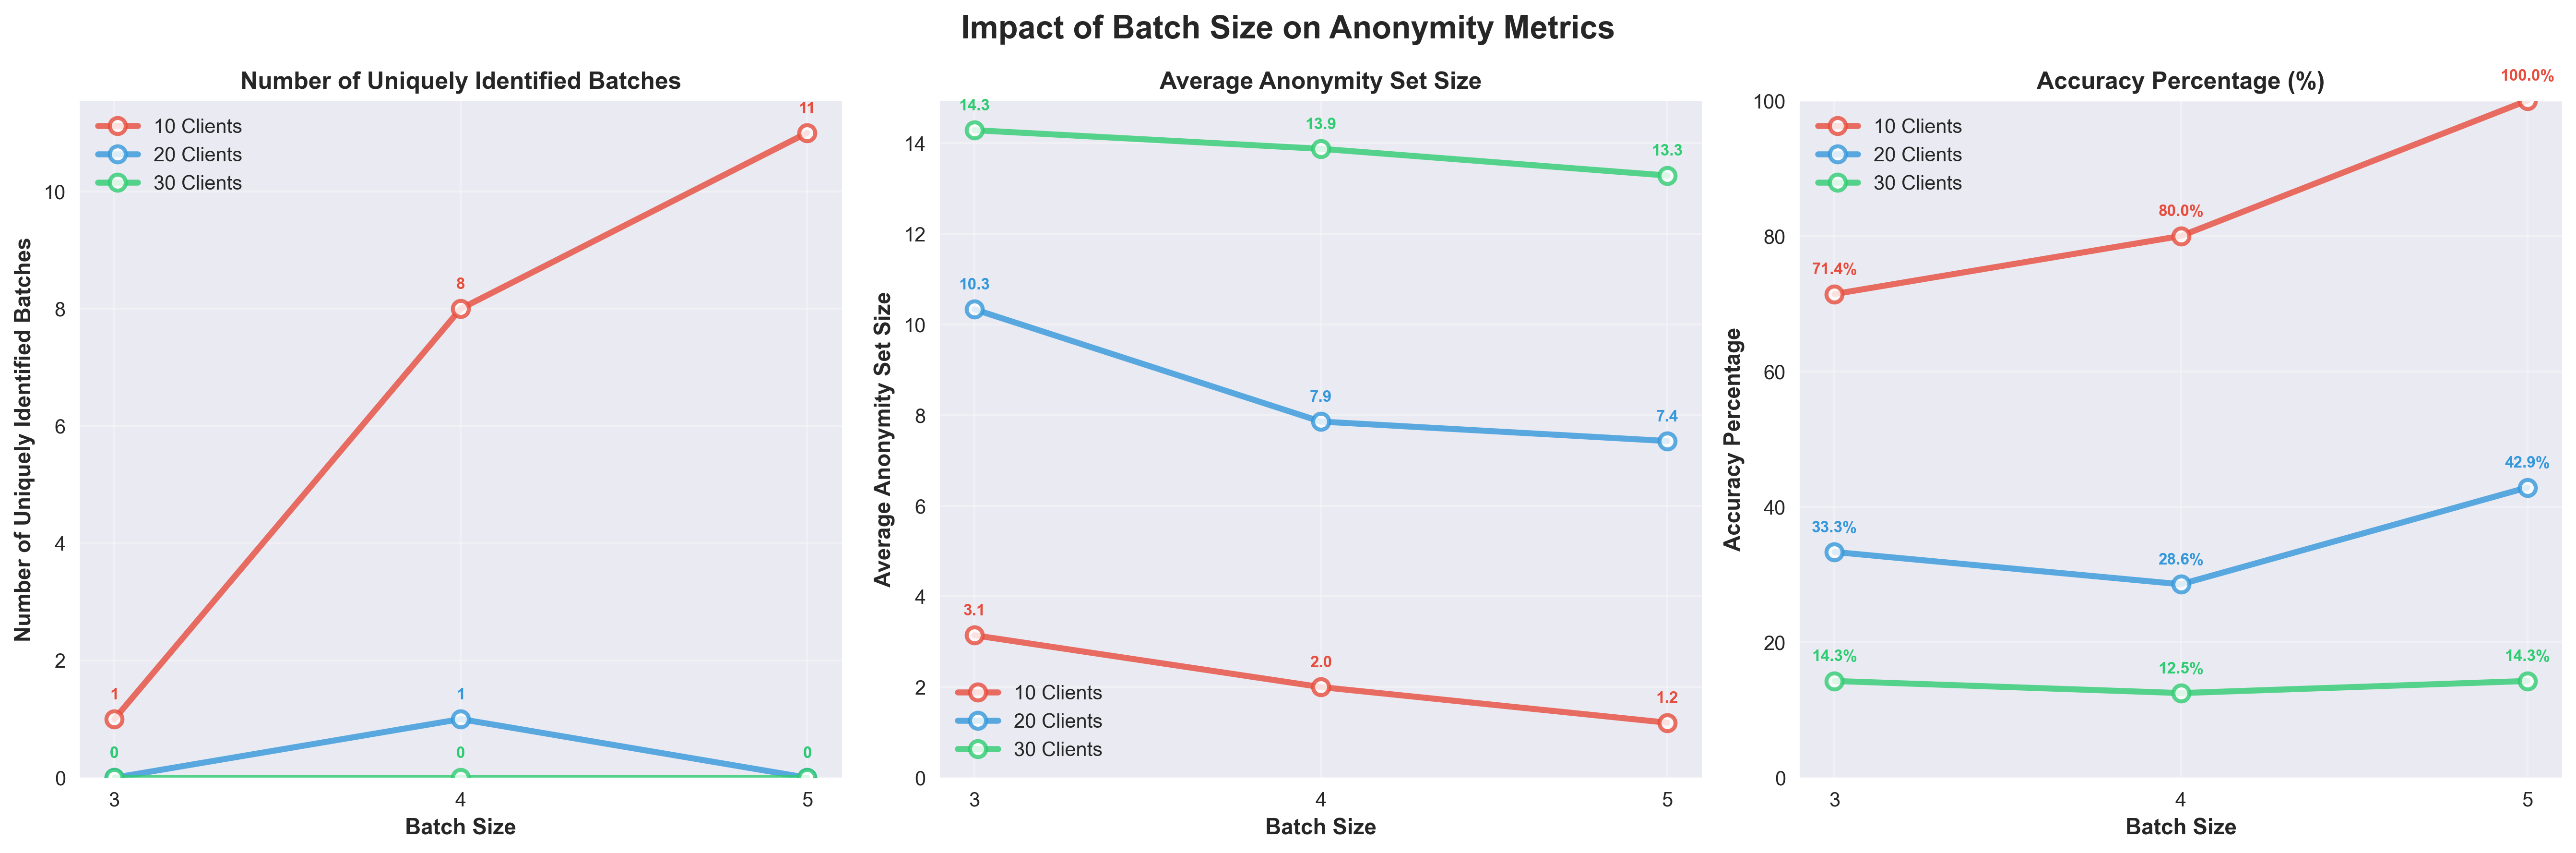
\includegraphics[width=\textwidth]{diagrams/batch_size_analysis_combined.png}
\caption{Impact of batch size on various anonymity metrics across 
different numbers of clients (10, 20, and 30 clients). 
The plots show how batch size affects the number of uniquely 
identified batches, average anonymity set size, and accuracy percentage.}
\label{fig:batchsize_analysis}
\end{figure*}

\begin{figure*}[!htb]
\centering
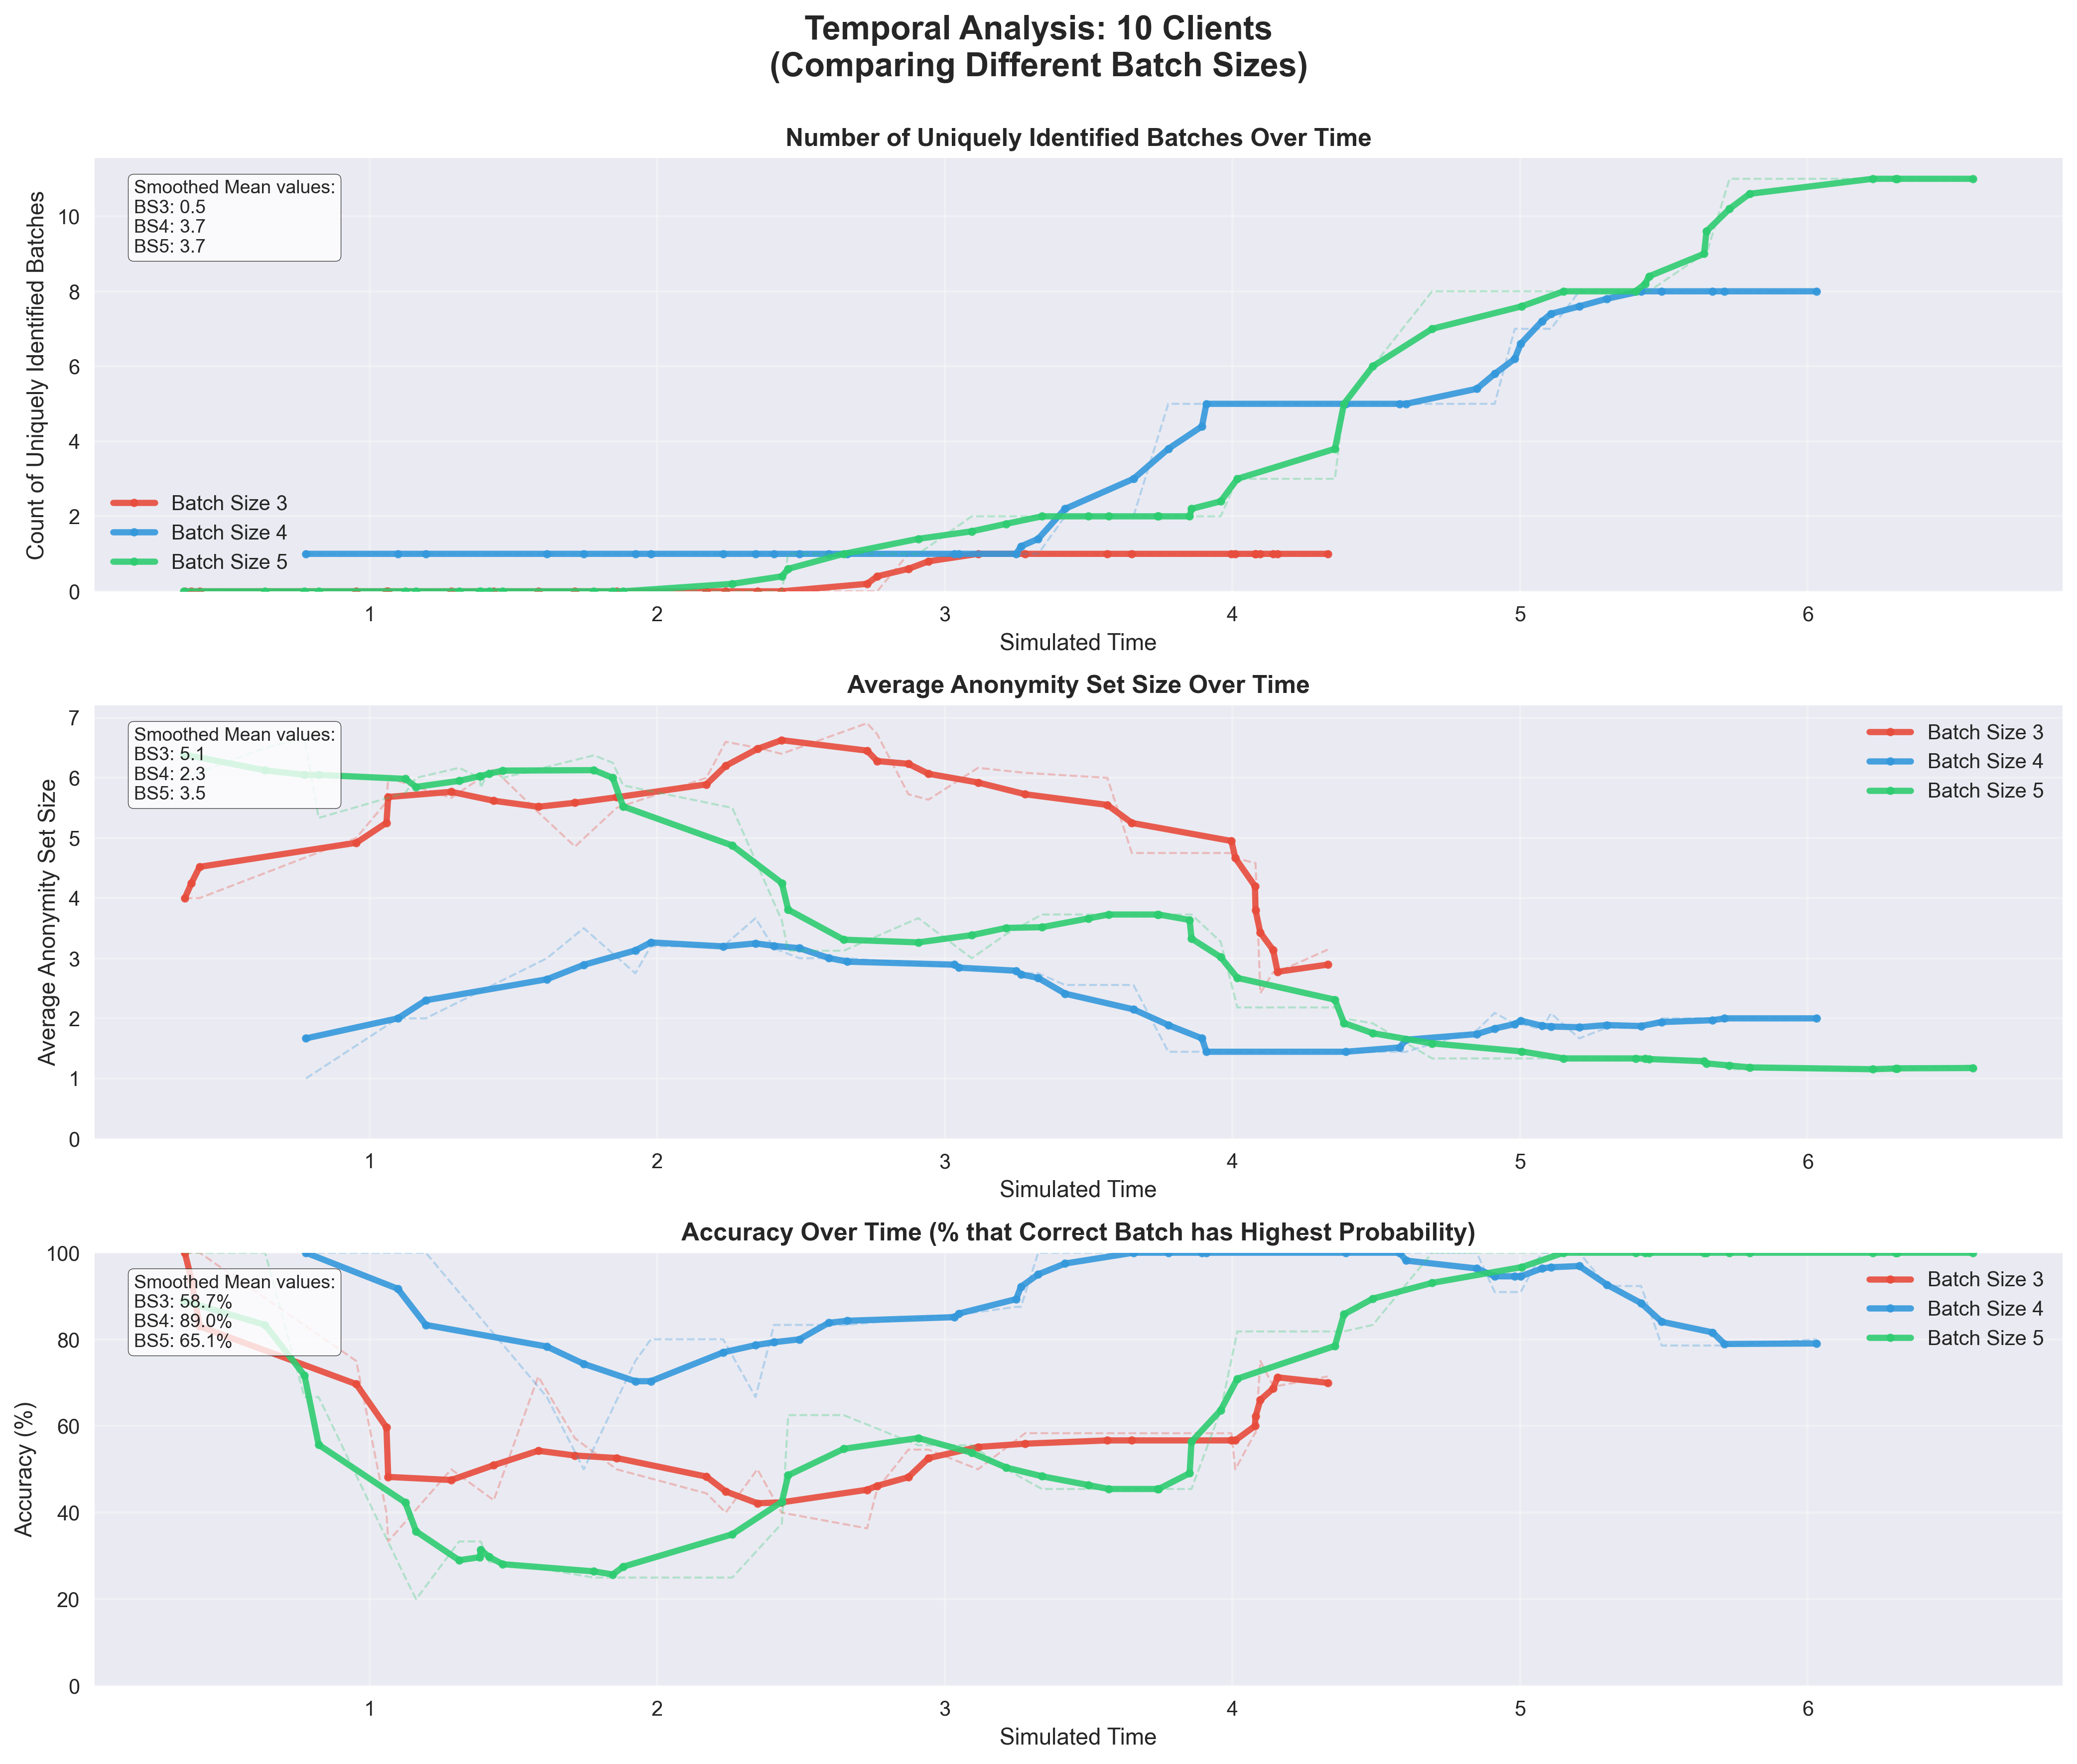
\includegraphics[width=\textwidth]{diagrams/temporal_5_smoothed_10_clients.png}
\caption{Temporal analysis of anonymity metrics for 10 clients across different batch sizes (3, 4, and 5).}
\label{fig:temporal_analysis_10}
\end{figure*}

\begin{figure*}[!htb]
\centering
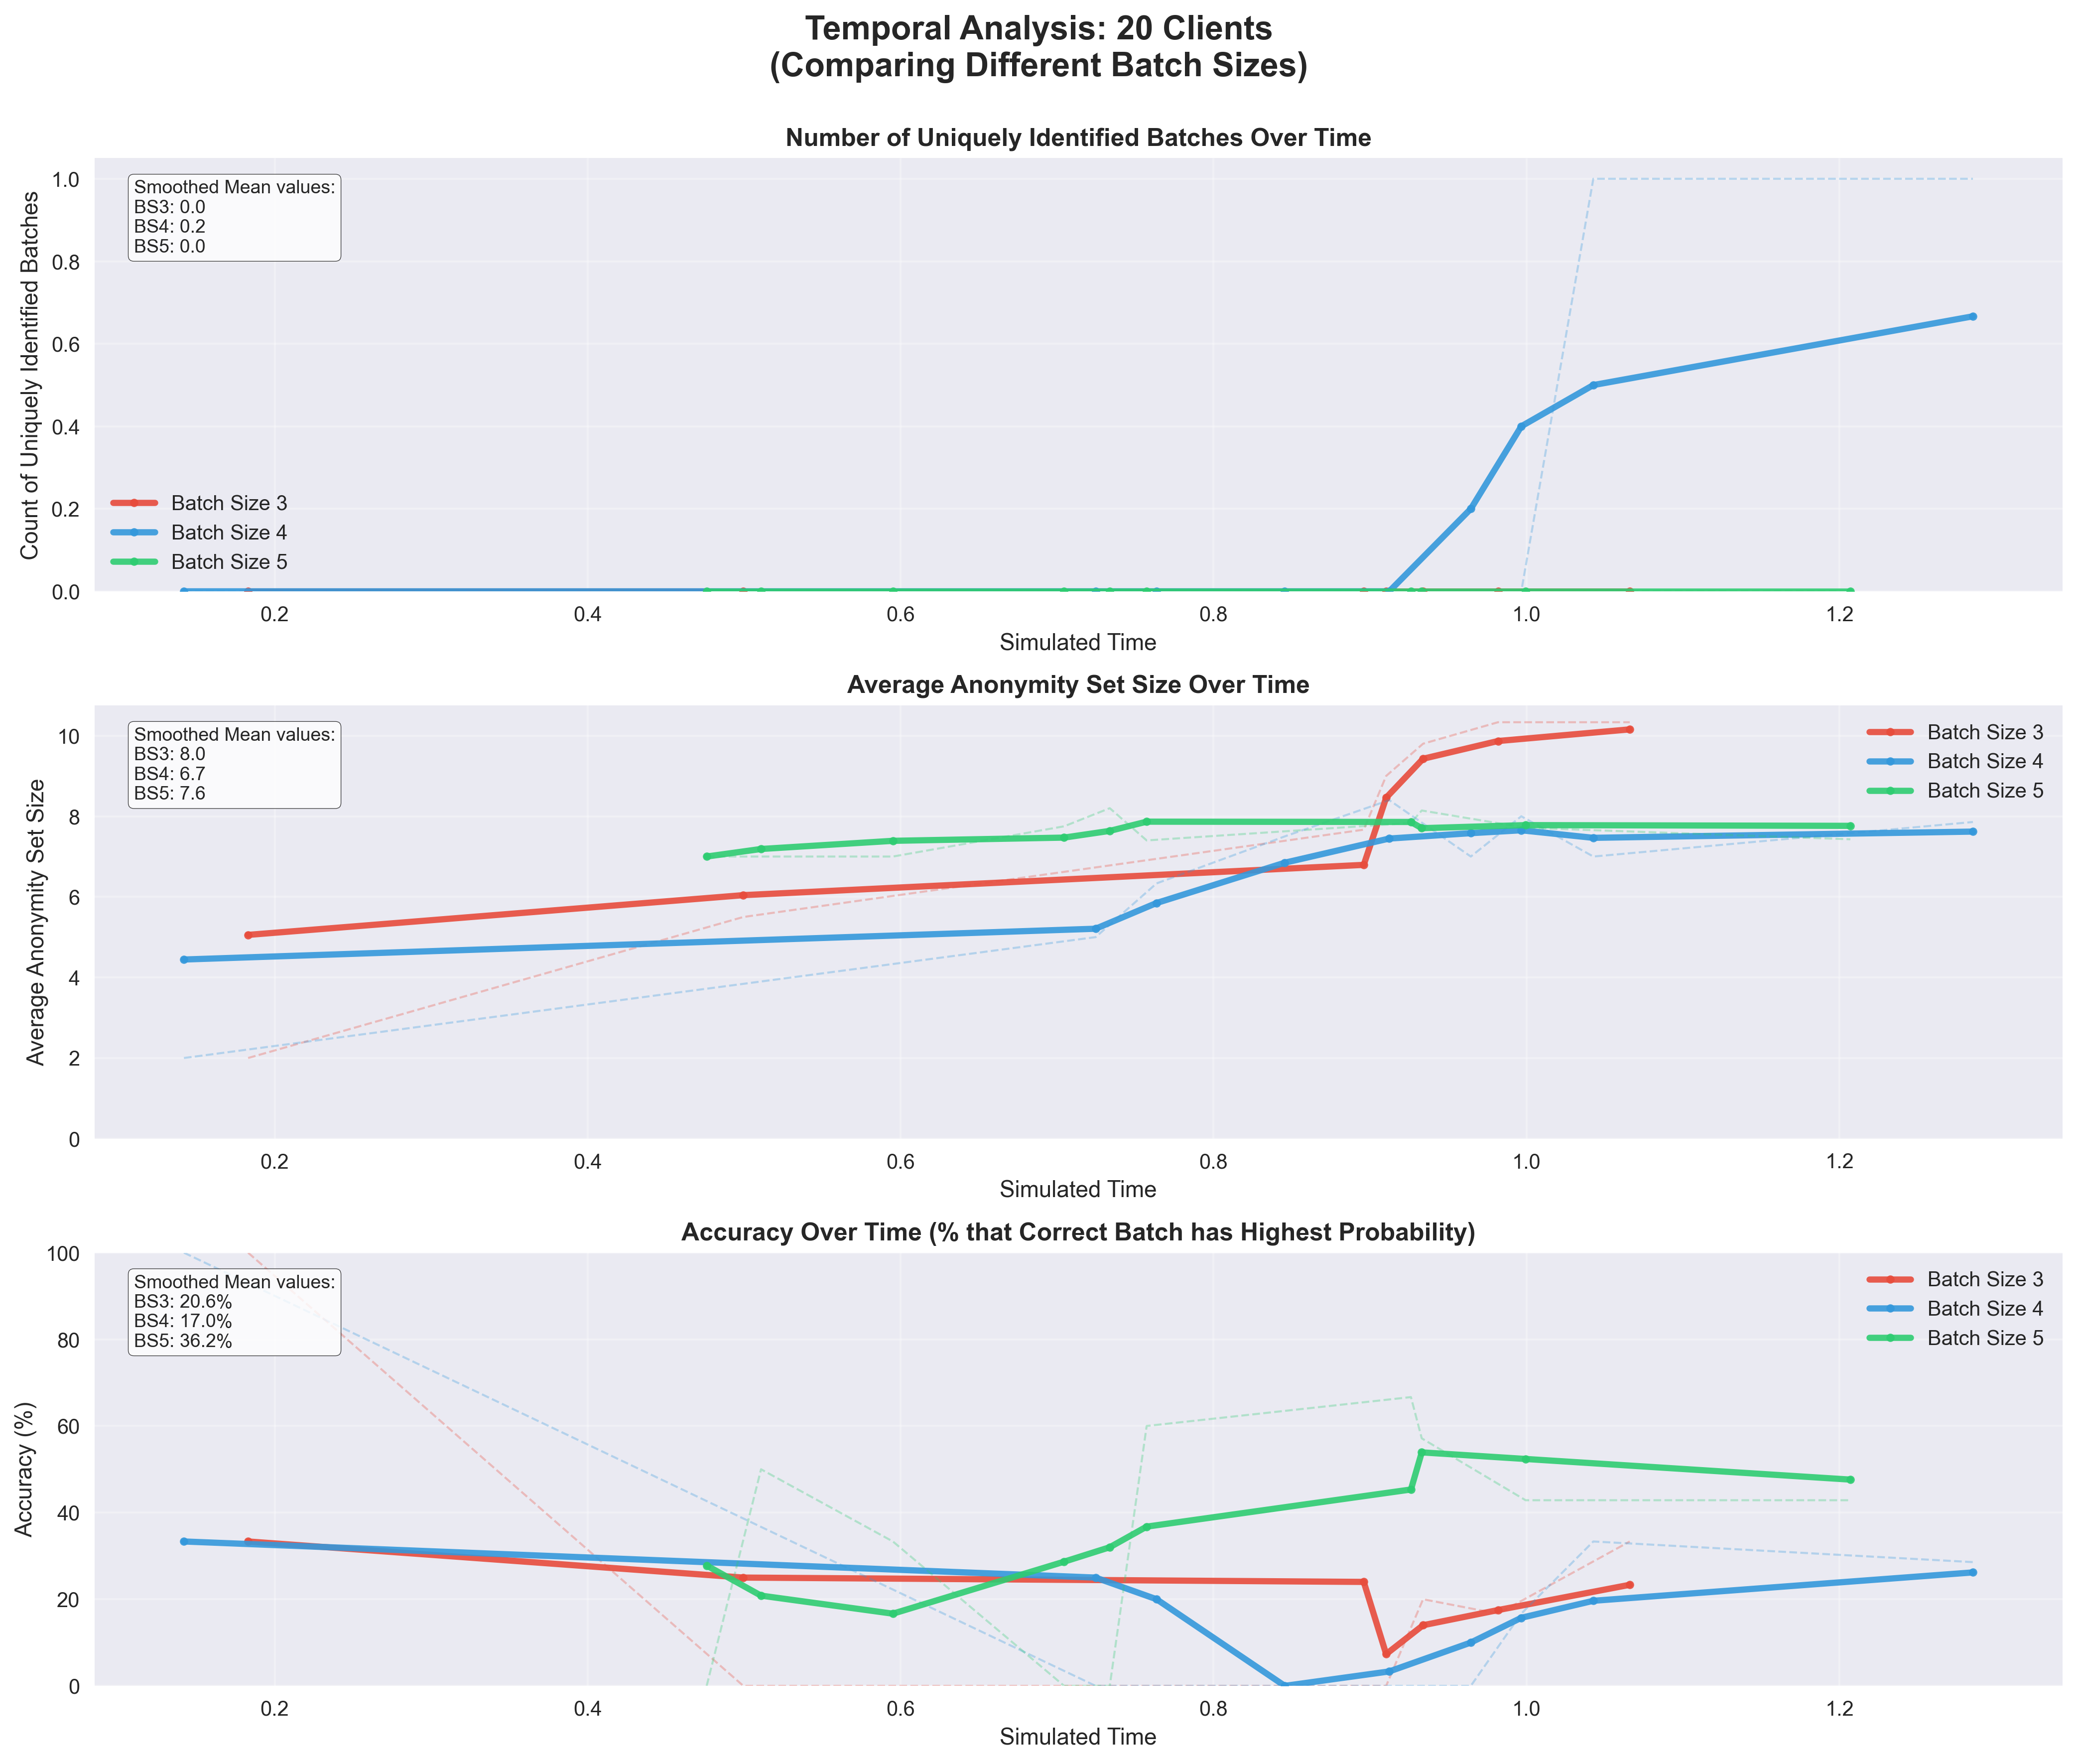
\includegraphics[width=\textwidth]{diagrams/temporal_5_smoothed_20_clients.png}
\caption{Temporal analysis of anonymity metrics for 20 clients across different batch sizes (3, 4, and 5).}
\label{fig:temporal_analysis_20}
\end{figure*}

\begin{figure*}[!htb]
\centering
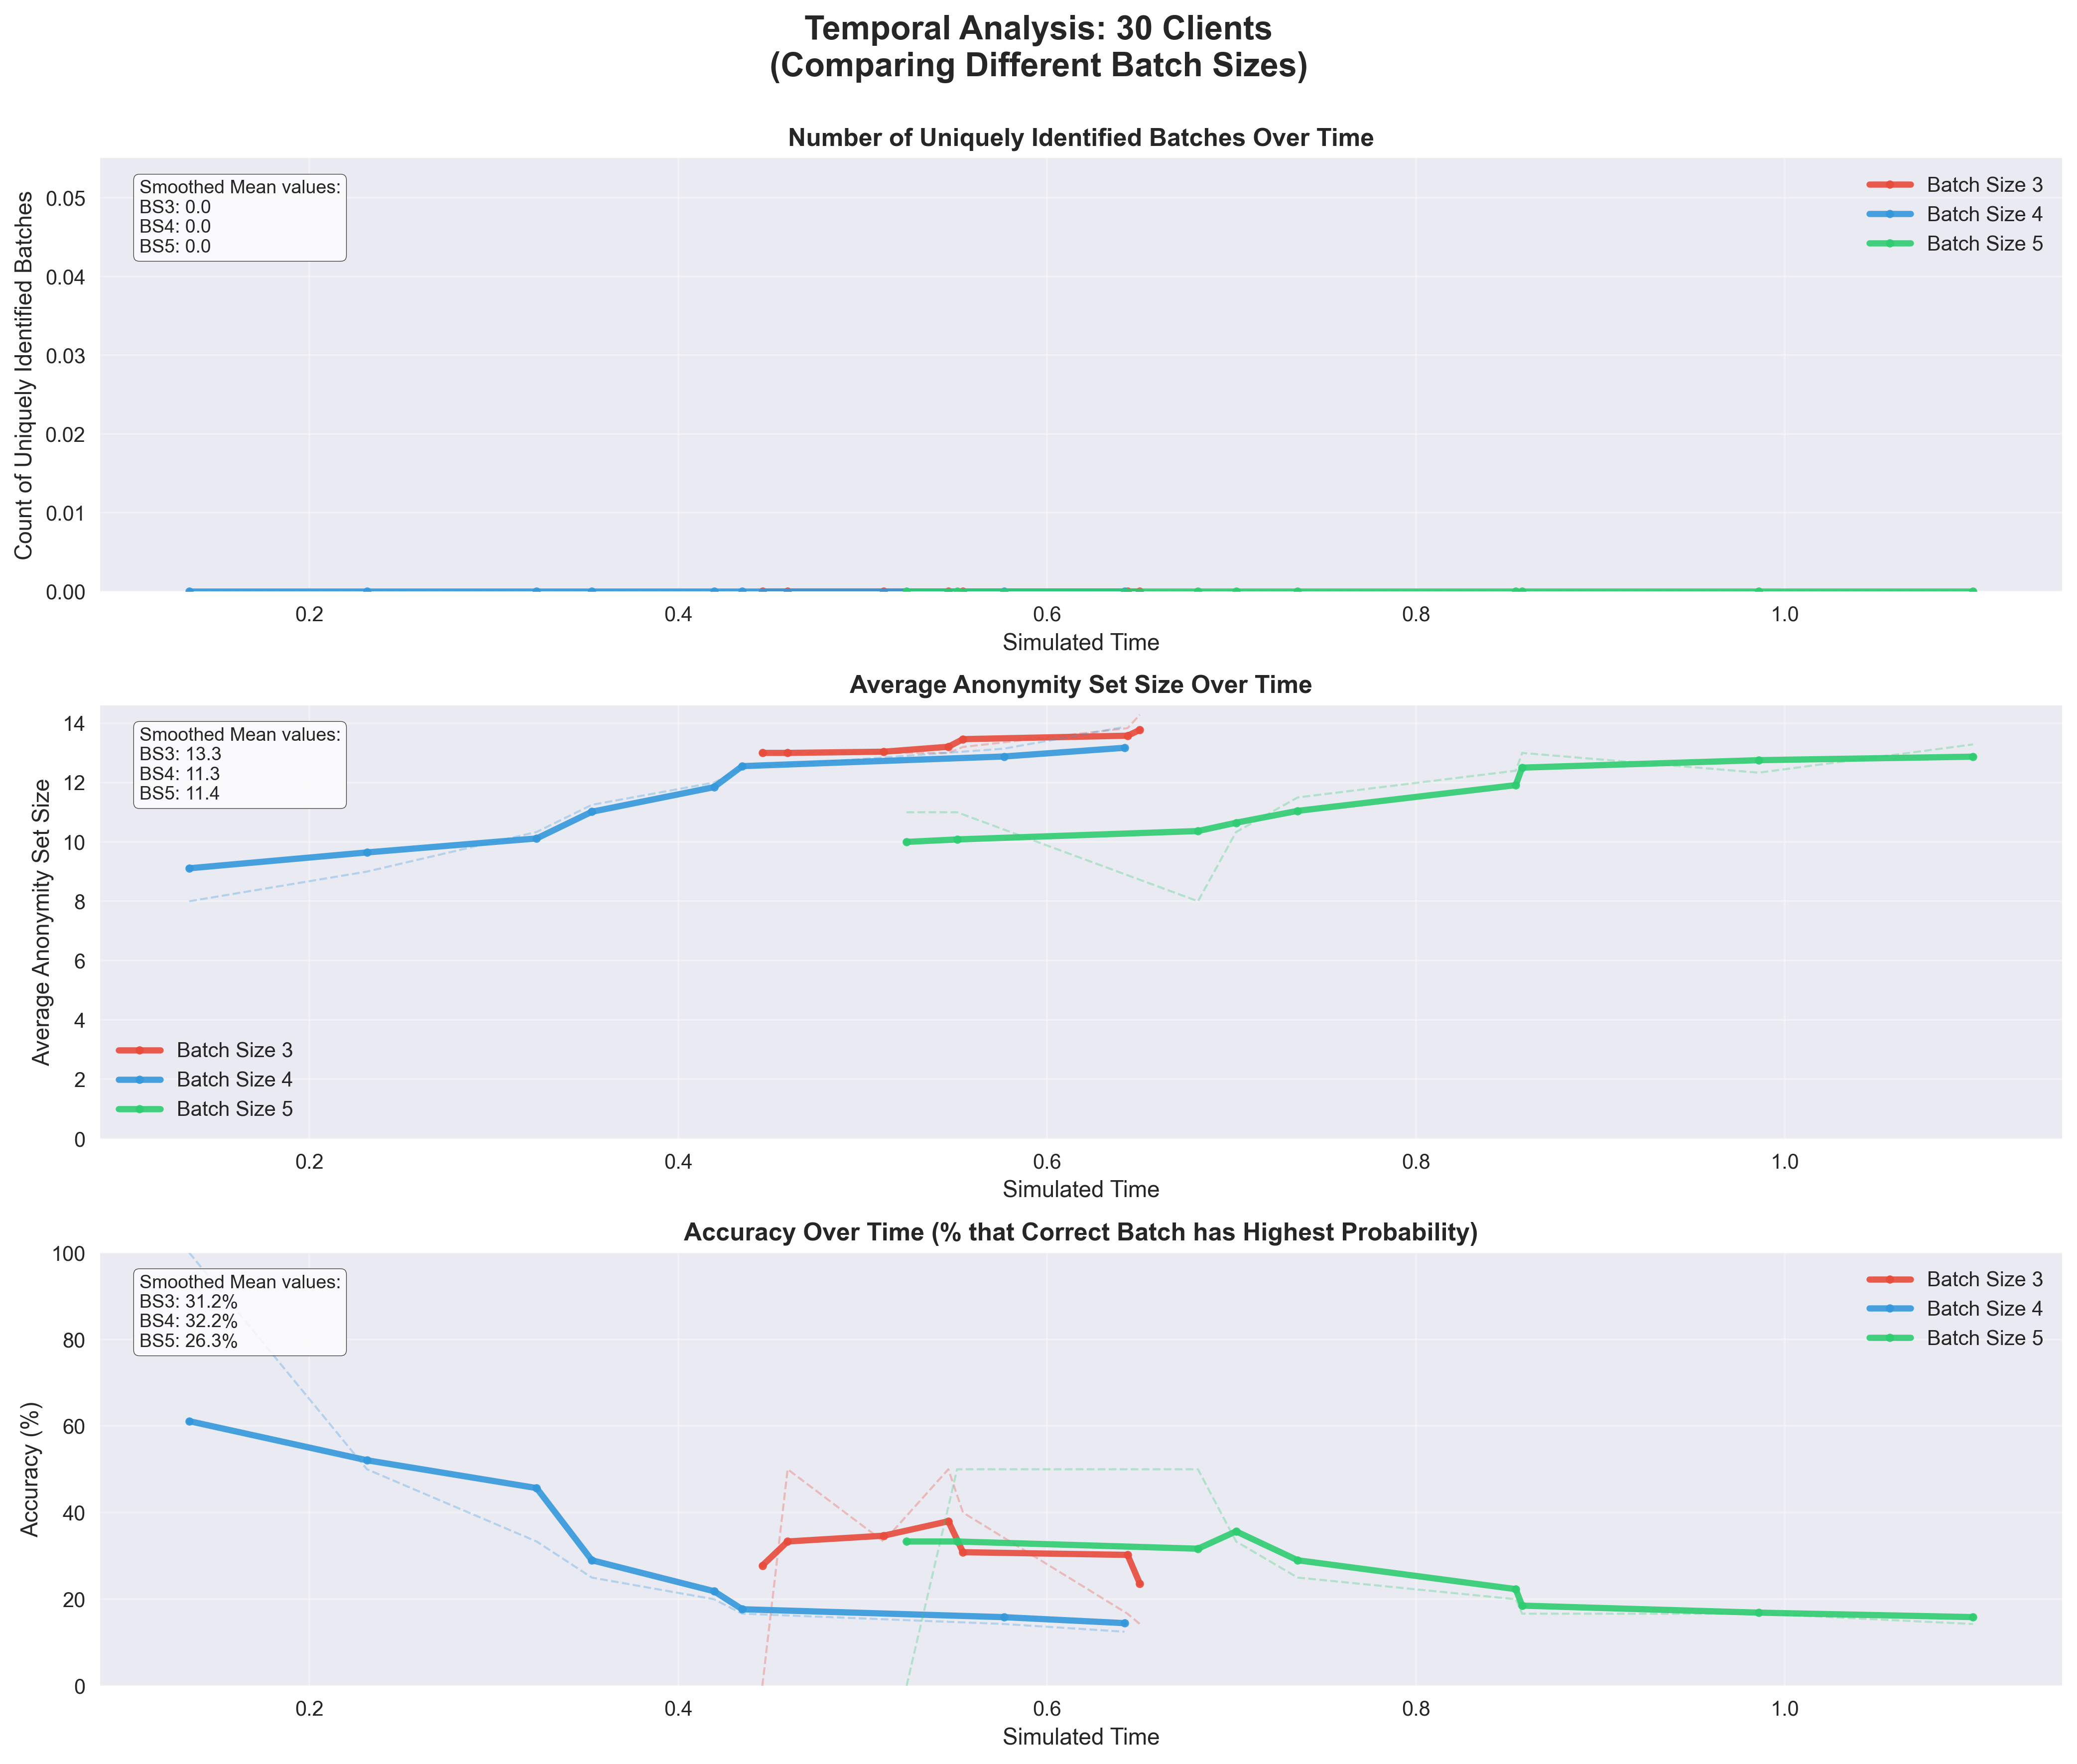
\includegraphics[width=\textwidth]{diagrams/temporal_5_smoothed_30_clients.png}
\caption{Temporal analysis of anonymity metrics for 30 clients across different batch sizes (3, 4, and 5).}
\label{fig:temporal_analysis_30}
\end{figure*}

\begin{figure*}[!htb]
\centering
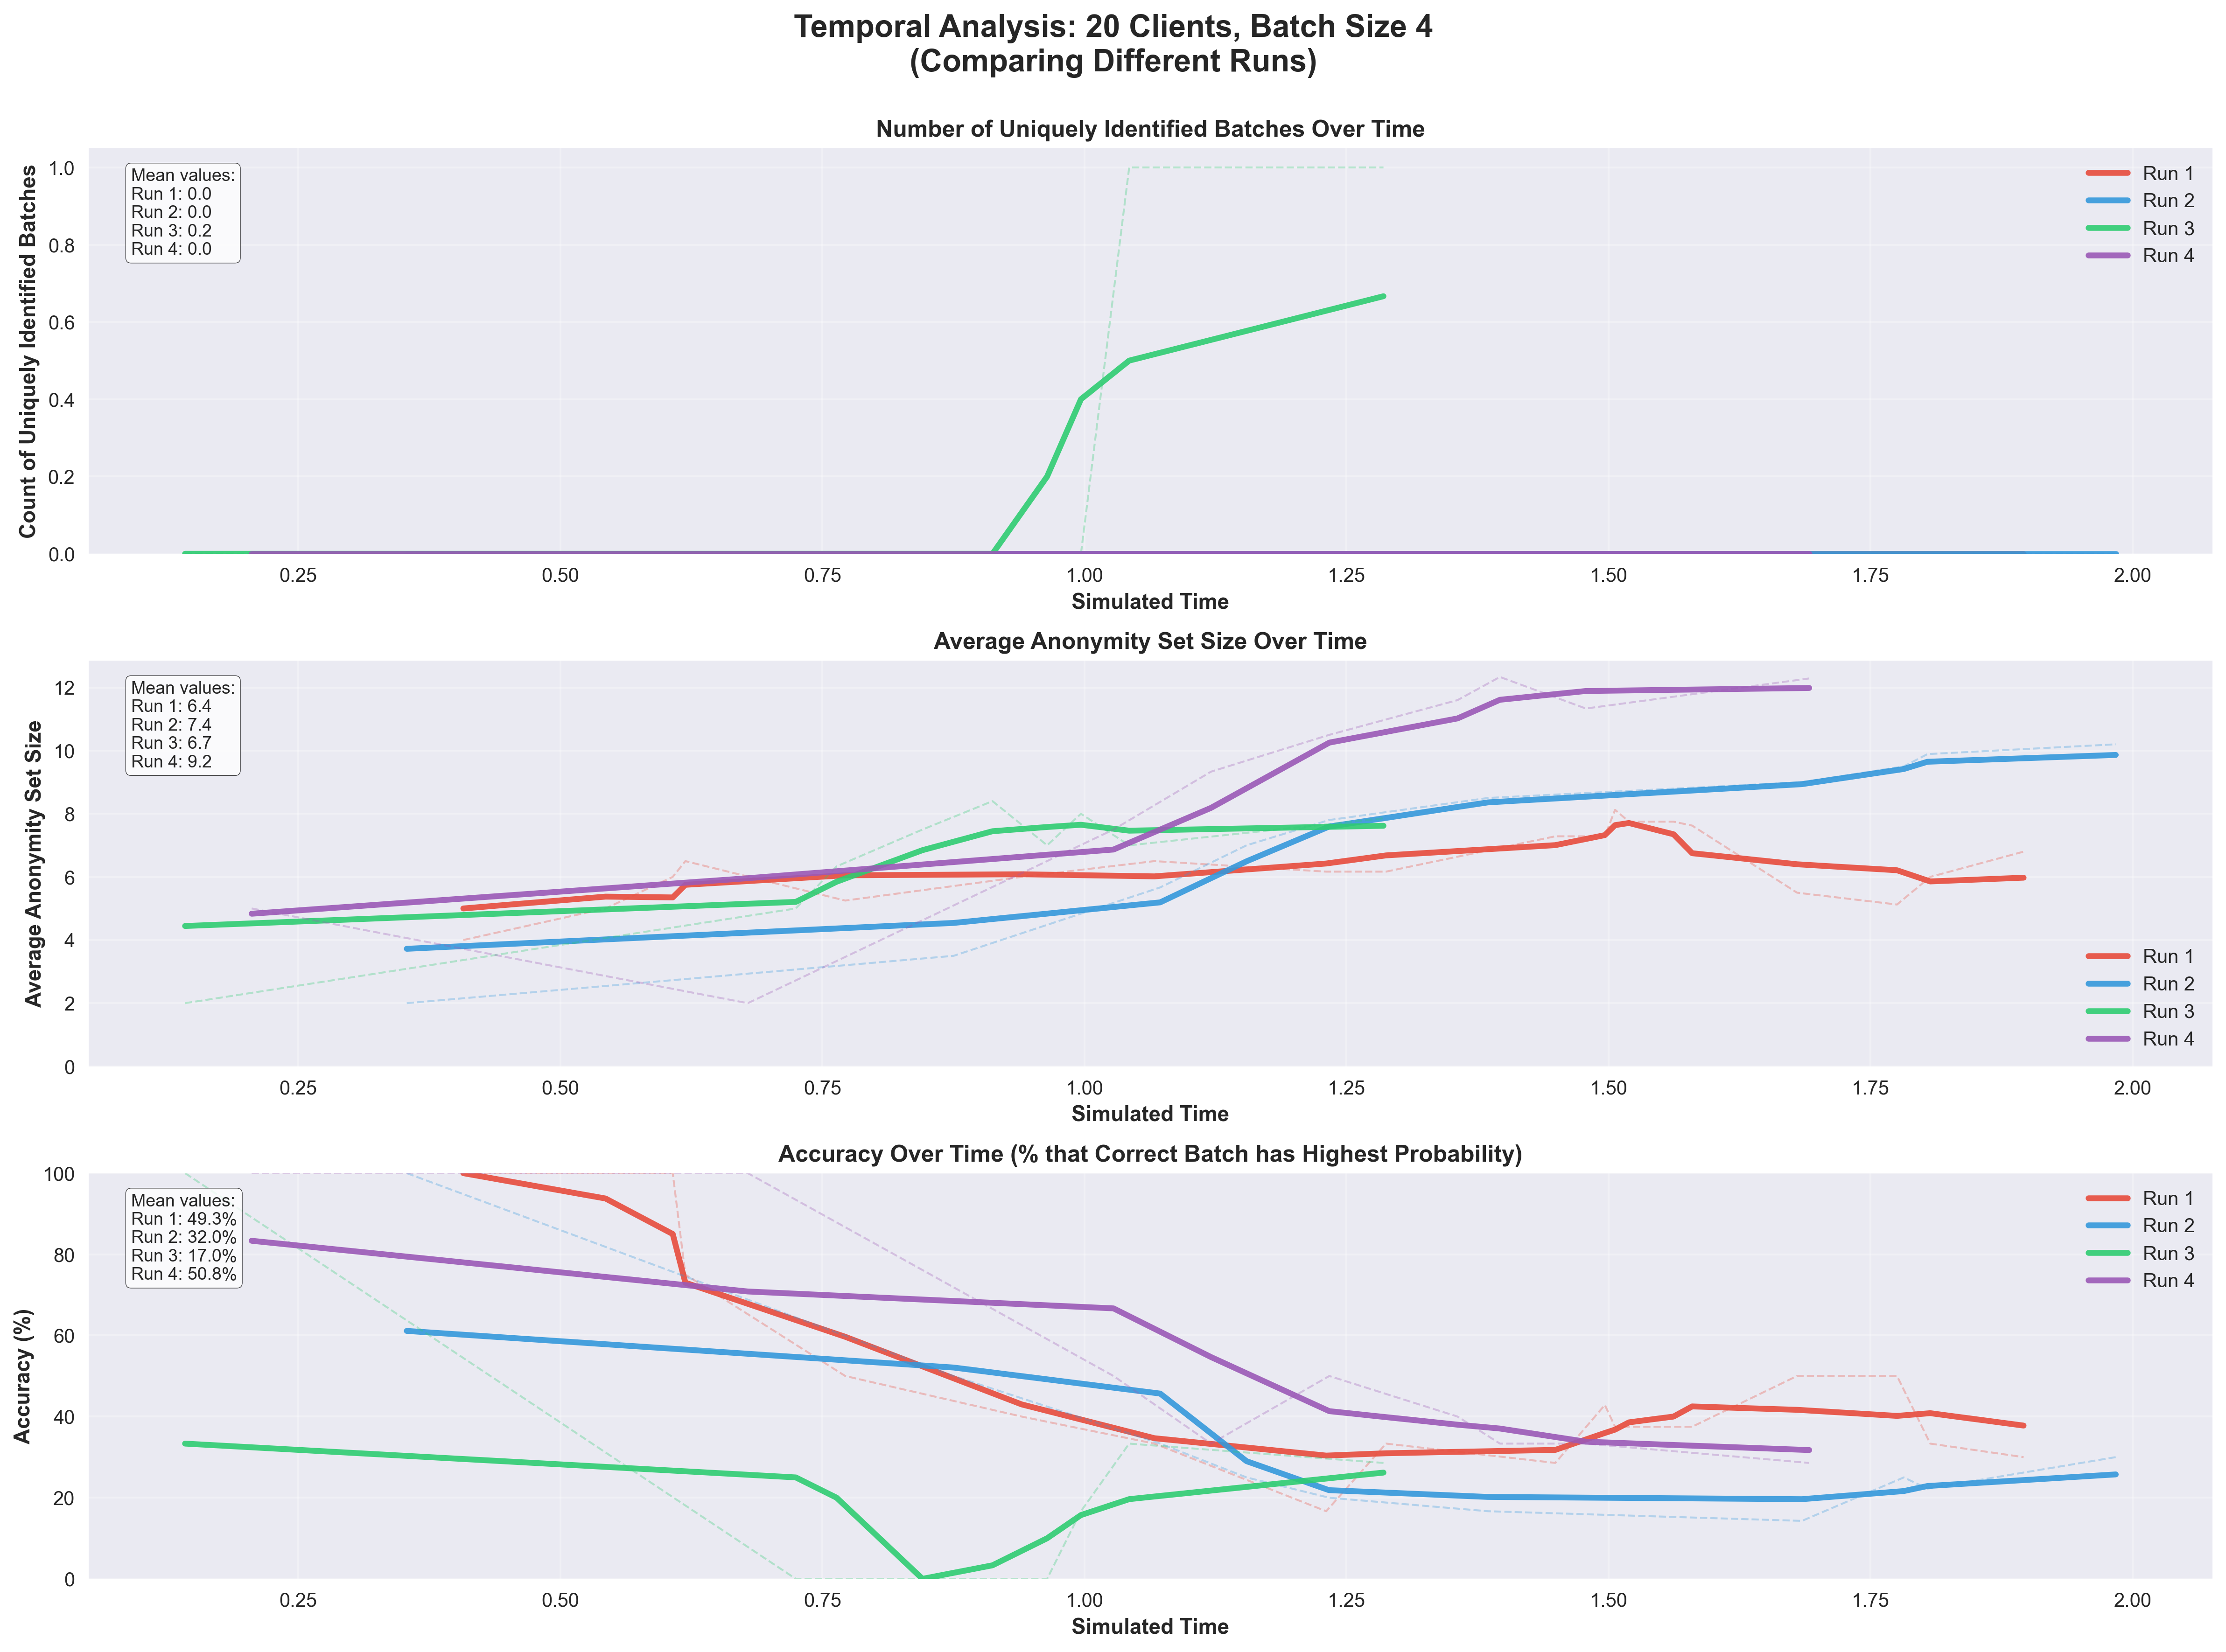
\includegraphics[width=\textwidth]{diagrams/temporal_20client_4batch_runs.png}
\caption{Reproducibility analysis showing temporal evolution of anonymity metrics across four independent simulation runs with identical parameters (20 clients, batch size 4).}
\label{fig:temporal_analysis_20_4_runs}
\end{figure*}

\subsection{Conclusion}
% \textbf{Conclusion:} 
It is important to note that due to computational limitations 
and the exponential complexity of the batch matching algorithm, 
our evaluation is based on a limited set of experimental runs. 
The patterns observed in this study should be interpreted with 
caution, as they represent only a small sample of the possible 
parameter space.

The computational complexity of enumerating all valid permutations 
scales poorly with both the number of clients and batch size, 
limiting our ability to conduct extensive statistical analysis. 
Additionally, the single-run approach for most configurations 
prevents us from establishing statistical significance or 
confidence intervals for our observations.

Future work should focus on developing more efficient algorithms 
that can handle larger parameter spaces and enable comprehensive 
statistical evaluation of anonymity guarantees under various 
operational conditions.

\end{document}